\section{Aplicación de estándares sobre el proyecto}

	\subsection{DCL51-CPP. No declare ni defina un identificador reservado}

		\subsubsection{Enlace al sitio web del estándar seleccionado}
		
			\paragraph{}\url{https://wiki.sei.cmu.edu/confluence/display/cplusplus/DCL51-CPP.+Do+not+declare+or+define+a+reserved+identifier}
		
		\subsubsection{Explicación sobre su utilidad}
		
			\paragraph{}El estándar de C++ (ISO/IEC 14882-2014) que hace referencia a los nombres reservados especifica las siguientes reglas:
			
			\begin{itemize}
				\item "\textit{Una unidad de traducción que incluye un encabezado de biblioteca estándar no debe \#define o \#undef nombres declarados en ningún encabezado de biblioteca estándar.}
				\item \textit{Una unidad de traducción no debe \#define o \#undef nombres léxicamente idénticos a palabras clave, a los identificadores enumerados en la Tabla 3, o a los atributos-tokens descritos en 7.6.}
				\item \textit{Cada nombre que contenga un guión bajo doble \_ \_ o comience con un guión bajo seguido de una letra mayúscula está reservado a la implementación para cualquier uso.}
				\item \textit{Cada nombre que comienza con un guión bajo se reserva para la implementación para su uso como nombre en el espacio de nombres global.}
				\item \textit{Cada nombre declarado como un objeto con enlace externo en un encabezado está reservado a la implementación para designar ese objeto de biblioteca con enlace externo, tanto en el espacio de nombres estándar como en el espacio de nombres global.}
				\item \textit{Cada firma de función global declarada con enlace externo en un encabezado está reservada a la implementación para designar esa firma de función con enlace externo.}
				\item \textit{Cada nombre de la biblioteca C estándar declarado con enlace externo está reservado a la implementación para su uso como un nombre con enlace C externo, tanto en el espacio de nombres estándar como en el espacio de nombres global.}
				\item \textit{Cada firma de función de la biblioteca C estándar declarada con enlace externo está reservada a la implementación para su uso como firma de función con enlace externo C y externo C++, o como nombre del ámbito del espacio de nombres en el espacio de nombres global.}
				\item \textit{Para cada tipo T de la biblioteca C estándar, los tipos ::T y std::T están reservados para la implementación y, cuando se defina, ::T será idéntico a std::T.}
				\item \textit{Los identificadores de sufijos literales que no comienzan con un guión bajo están reservados para una futura estandarización.}"
			\end{itemize}
		
			\paragraph{}Los identificadores y nombres de atributos a los que se hace referencia en el extracto anterior son override, final, alignas, carry\_dependency, deprecated y noreturn. Ningunos otros identificadores están reservados.
			
			\paragraph{}Declarar o definir identificadores en un contexto en el que estén reservados derivará en un comportamiento indefinido o impredecible. Para evitar esto, siempre hay que evitar reservar o definir identificadores que estén reservados.
		
		\subsubsection{Aplicación del estándar al proyecto}
		
			\paragraph{}Nuestro proyecto cumple perfectamente con el estándar, ya que no hace uso de ningún identificador reservado. Uno de los ejemplos de las reglas definidas en el apartado anterior es la nomenclatura de las cabeceras de los archivos, a continuación una captura de pantalla de una de ellas:
			
			\begin{figure}[H]
				\centering
				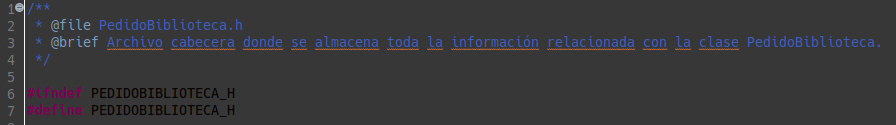
\includegraphics[scale=0.5]{img/captura40.png}
				\caption{Captura de pantalla del cumplimiento del estándar DCL51-CPP.}
				\label{captura40}
			\end{figure}
		
			\paragraph{}Otro ejemplo de cumplimiento del estándar es el uso del identificador T en la implementación de las plantillas del programa. A continuación, una captura de pantalla de dicho uso:
			
			\begin{figure}[H]
				\centering
				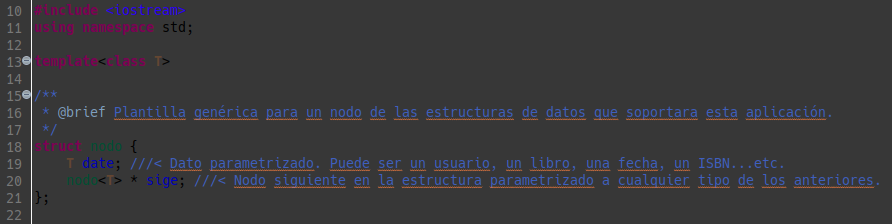
\includegraphics[scale=0.5]{img/captura41.png}
				\caption{Captura de pantalla del cumplimiento del estándar DCL51-CPP.}
				\label{captura41}
			\end{figure}
		
			\paragraph{}Estos son los dos ejemplos más claros de cumplimiento del estándar. No podemos mostrar más capturas de pantalla ya que, al no hacer uso de identificadores reservados, no podemos mostrar las correcciones de los incumplimientos.

	\subsection{DCL52-CPP. Nunca califique un tipo de referencia con constante o volátil}
	
		\subsubsection{Enlace al sitio web del estándar seleccionado}
		
			\paragraph{}\url{https://wiki.sei.cmu.edu/confluence/display/cplusplus/DCL52-CPP.+Never+qualify+a+reference+type+with+const+or+volatile}
		
		\subsubsection{Explicación sobre su utilidad}
		
			\paragraph{}Como sabemos de cursos anteriores, C++ no permite modificar el valor de una variable que haya sido calificada con constante (const). 
			
			\paragraph{}En el caso de objetos que sea referenciados, es decir, utilizando el caracter reservado '$\&$' se puede cometer el error de escribir la expresión de la siguiente forma: "$char$ $const\&$ $p$", C++ ignora o prohibe la asignación de referencia a la palabra reservada "const". Este hecho puede desencadenar en escrituras accidentales en la variable constante, probocando resultados no esperados en la ejecución del programa.
			
			\paragraph{}Para que la expresión fuera correcta, debería escribirse de una de las siguientes formas: "$const$ $char$ $\&p$" ó "$char$ $const$ $\&p$"
		
		\subsubsection{Aplicación del estándar al proyecto}
		
			\paragraph{}En nuestro proyecto hacemos uso repetidas veces de expresiones con referencias de este tipo, y en todas ellas respetamos la sintaxis que se describe en el presente estándar.
			
			\paragraph{}A continuación, presentamos capturas de pantalla de alguna de las expresiones que se encuentran en el código fuente a modo de ejemplo:
			
			\begin{figure}[H]
				\centering
				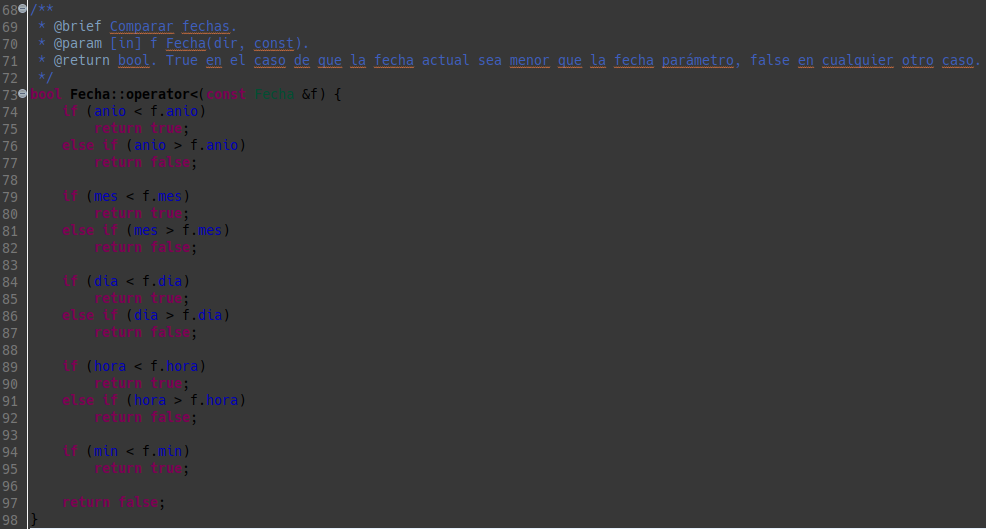
\includegraphics[scale=0.45]{img/captura38.png}
				\caption{Captura de pantalla del cumplimiento del estándar DCL52-CPP.}
				\label{captura38}
			\end{figure}
		
			\begin{figure}[H]
				\centering
				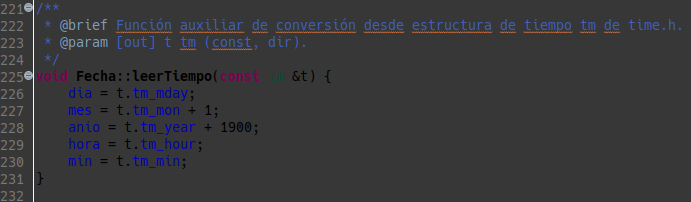
\includegraphics[scale=0.6]{img/captura39.png}
				\caption{Captura de pantalla del cumplimiento del estándar DCL52-CPP.}
				\label{captura39}
			\end{figure}

	\subsection{DCL59-CPP. No defina un espacio de nombres sin nombre en un archivo de encabezado.}
	
		\subsubsection{Enlace al sitio web del estándar seleccionado}
			
			\paragraph{}\url{https://wiki.sei.cmu.edu/confluence/display/cplusplus/DCL59-CPP.+Do+not+define+an+unnamed+namespace+in+a+header+file}
		
		\subsubsection{Explicación sobre su utilidad}
		
			\paragraph{}El código C++ de calidad de producción utiliza con frecuencia archivos de encabezado como medio para compartir código entre unidades de traducción. Un archivo de encabezado es cualquier archivo que se inserta en una unidad de traducción a través de una directiva. No defina un espacio de nombres sin nombre en un archivo de encabezado. Cuando se define un espacio de nombres sin nombre en un archivo de encabezado, puede dar lugar a resultados sorprendentes. Debido al vínculo interno predeterminado, cada unidad de traducción definirá su propia instancia única de los miembros del espacio de nombres sin nombre que se usan en ODR dentro de esa unidad de traducción. Esto puede causar resultados inesperados, hinchar el ejecutable resultante o desencadenar inadvertidamente el comportamiento indefinido debido a infracciones de una regla de una definición.
		
		\subsubsection{Aplicación del estándar al proyecto}
		
			\paragraph{}Los espacios de nombres sin nombre se usan para definir un espacio de nombres que es único para la unidad de traducción, donde los nombres contenidos tienen vinculación interna de forma predeterminada.
			
			\begin{figure}[H]
				\centering
				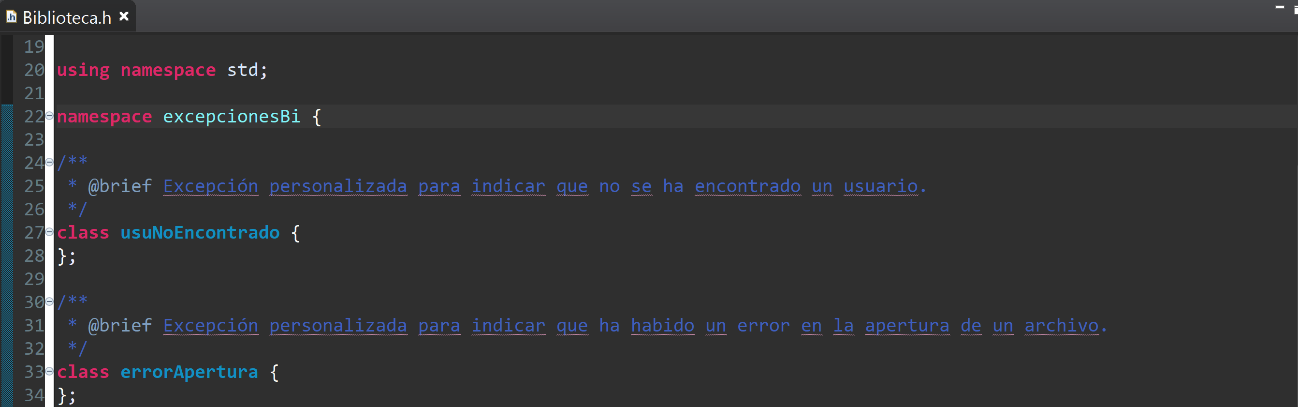
\includegraphics[scale=0.8]{img/img1.png}
				\caption{Captura de pantalla del cumplimiento del estándar DCL59-CPP.}
				\label{img1}
			\end{figure}
			
			\paragraph{}Aquí observamos como en un archivo cabecera al incluir un nuevo espacio de nombres, se le ha tenido que poner un nombre distinto para no confundir a la unidad de traducción. En este caso el nombre ofrecido ha sido el de “excepcionesBi”.
			
			\begin{figure}[H]
				\centering
				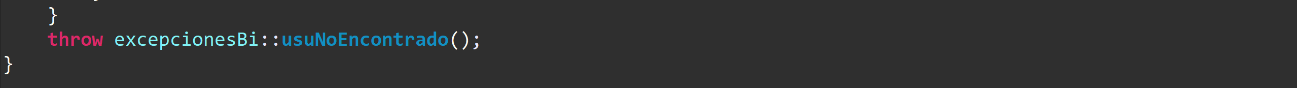
\includegraphics[scale=0.8]{img/img2.png}
				\caption{Captura de pantalla del cumplimiento del estándar DCL59-CPP.}
				\label{img2}
			\end{figure}
			
			\paragraph{}Así puede ser perfectamente referenciado desde el .cpp de dicho archivo Biblioteca como podemos ver en la imagen:
	
	\subsection{MEM51-CPP. Desasignar correctamente la memoria asignada a los objetos dinámicamente.}
	
		\subsubsection{Enlace al sitio web del estándar seleccionado}
		
			\paragraph{}\url{https://wiki.sei.cmu.edu/confluence/display/cplusplus/MEM51-CPP.+Properly+deallocate+dynamically+allocated+resources}
		
		\subsubsection{Explicación sobre su utilidad}
		
			\paragraph{}La desasignación de un puntero que no está asignado dinámicamente (incluidos los punteros no dinámicos devueltos por las llamadas a la ubicación new ()) es un comportamiento indefinido porque el valor del puntero no se obtuvo mediante una función de asignación. La desasignación de un puntero que ya se ha pasado a una función de desasignación es un comportamiento indefinido porque el valor del puntero ya no apunta a la memoria que se ha asignado dinámicamente.
			
			\paragraph{}Cuando new se llama a un operador como el resultado es una llamada a un operador sobre cargable con el mismo nombre, como operator new (). Estas funciones sobrecargables se pueden llamar directamente, pero tienen las mismas restricciones que sus contrapartes de operador. Es decir, llamar operator delete () y pasar un parámetro de puntero tiene las mismas restricciones que llamar al delete operador en ese puntero. Además, las sobrecargas están sujetas a la resolución del alcance, por lo que es posible (pero no permitido) llamar a un operador específico de clase para asignar un objeto, pero a un operador global para desasignar el objeto.
		
		\subsubsection{Aplicación del estándar al proyecto}
		
			\paragraph{}Aquí vemos como se llama al operador new ():
			
			\begin{figure}[H]
				\centering
				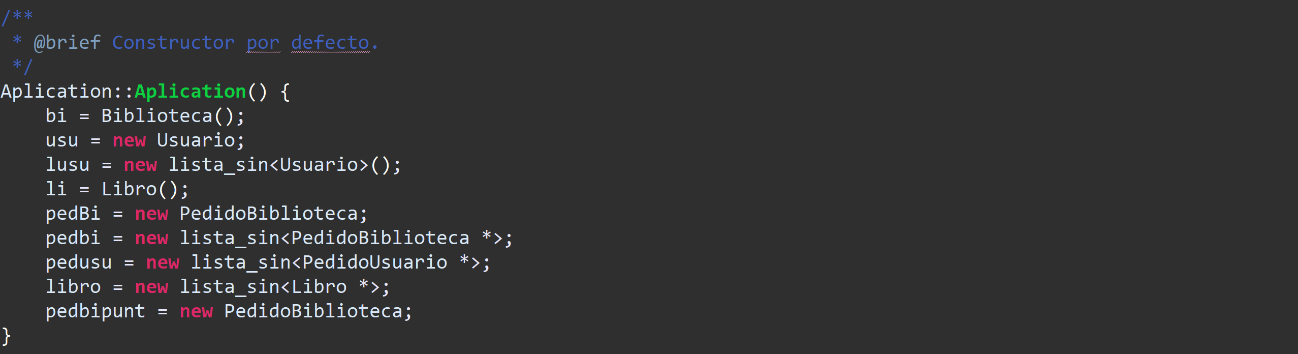
\includegraphics[scale=0.8]{img/img3.png}
				\caption{Captura de pantalla del cumplimiento del estándar MEM51-CPP.}
				\label{img3}
			\end{figure}
			
			\paragraph{}Para desasignar correctamente la memoria asignada dinámicamente a estos objetos observamos como en el destructor se hacen las llamadas correspondientes al operador delete () que es la contraparte de new () y además a la función de limpieza, que internamente hace también una llamada al operador delete ().
			
			\begin{figure}[H]
				\centering
				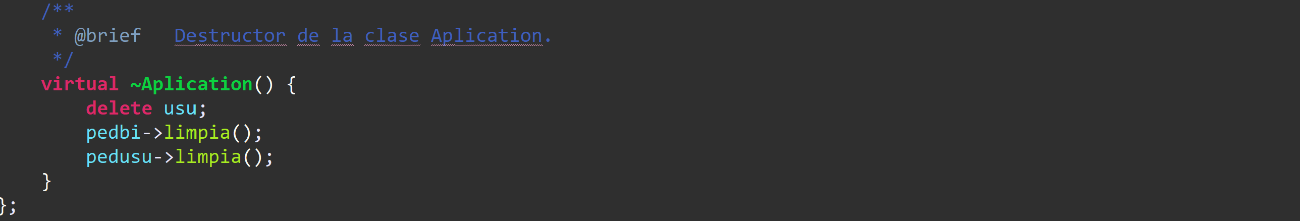
\includegraphics[scale=0.8]{img/img4.png}
				\caption{Captura de pantalla del cumplimiento del estándar DCL59-CPP.}
				\label{img4}
			\end{figure}
		
	\subsection{MEM52-CPP. Detectar errores de asignación de memoria}
	
		\subsubsection{Enlace al sitio web del estándar seleccionado}
		
			\paragraph{}\url{https://wiki.sei.cmu.edu/confluence/display/cplusplus/MEM52-CPP.+Detect+and+handle+memory+allocation+errors}
		
		\subsubsection{Explicación sobre su utilidad}
		
			\paragraph{}El operador de asignación de memoria predeterminado ::operator new (std::size\_t), lanza una excepción std::bad\_alloc si falla la asignación. Por lo tanto, no es necesario verificar si la llamada ::operator new(std::size\_t) da como resultado nullptr . La forma de ::operator new(std::size\_t, const std::nothrow\_t $\&$)no lanzar, no lanza una excepción si la asignación falla, sino que regresa nullptr. Los mismos comportamientos se aplican a las operator new [] versiones de ambas funciones de asignación. Además, el objeto de asignación predeterminado ( std::allocator) se usa  ::operator new(std::size\_t)para realizar asignaciones y debe tratarse de manera similar.
		
		\subsubsection{Aplicación del estándar al proyecto}

			\paragraph{}Por ejemplo, si no se ha podido asignar memoria para usu con el operador new (), aparte de las excepciones personalizadas que nos mostrarían un mensaje, es correcto que en el primer bloque catch se atrapara también esta excepción si acaso fallase la asignación.
			
			\begin{figure}[H]
				\centering
				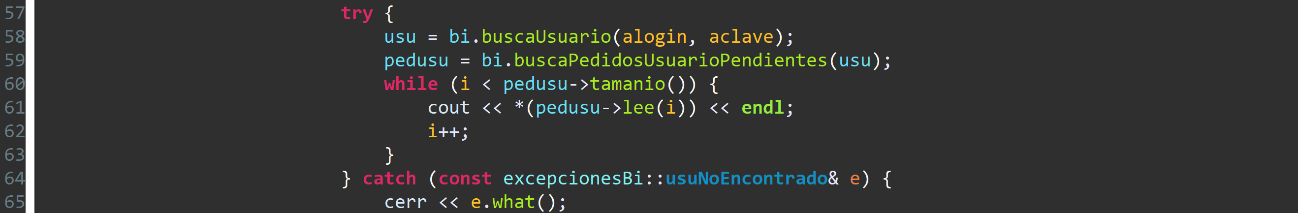
\includegraphics[scale=0.8]{img/img5.png}
				\caption{Captura de pantalla del incumplimiento del estándar MEM52-CPP.}
				\label{img5}
			\end{figure}
			
			\paragraph{}Una vez arreglado, se muestra ya en los catch la “bad\_alloc” si falla la asignación de memoria:
			
			\begin{figure}[H]
				\centering
				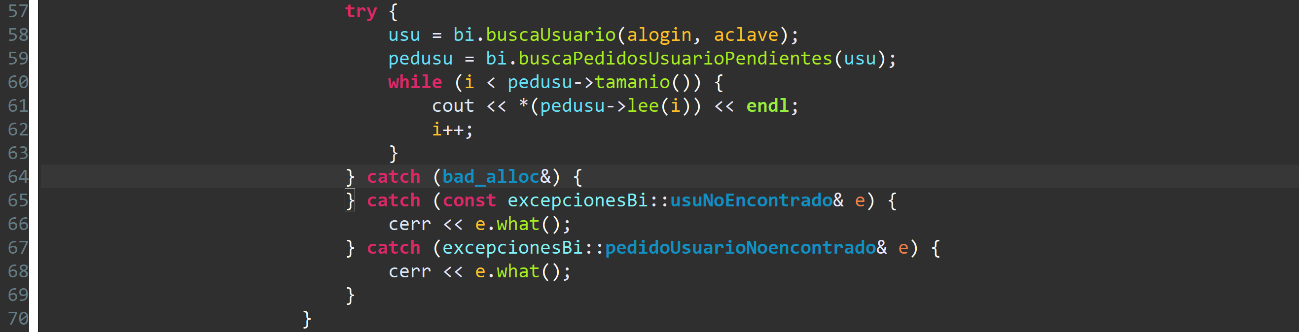
\includegraphics[scale=0.8]{img/img6.png}
				\caption{Captura de pantalla del cumplimiento del estándar MEM52-CPP.}
				\label{img6}
			\end{figure}
		
	\subsection{FIO50-CPP. No ingrese y elabore alternativamente desde un flujo sin una llamada de posicionamiento.}
	
		\subsubsection{Enlace al sitio web del estándar seleccionado}
		
			\paragraph{}\url{https://wiki.sei.cmu.edu/confluence/display/cplusplus/FIO50-CPP.+Do+not+alternately+input+and+output+from+a+file+stream+without+an+intervening+positioning+call}
		
		\subsubsection{Explicación sobre su utilidad}
		
			\paragraph{}Cuando se abre un archivo, tanto la entrada como la salida pueden realizarse en el flujo asociado. Sin embargo, la salida no será seguido directamente por la entrada sin una llamada de intervenir para la  fflush función o a una función de archivo de posicionamiento ( fseek,  fsetpos o rewind), y la entrada no será seguida directamente por la salida sin una llamada de intervención para una función de fichero de posicionamiento, a menos que la operación de entrada encuentra el final del archivo.
		
		\subsubsection{Aplicación del estándar al proyecto}
		
			\begin{figure}[H]
				\centering
				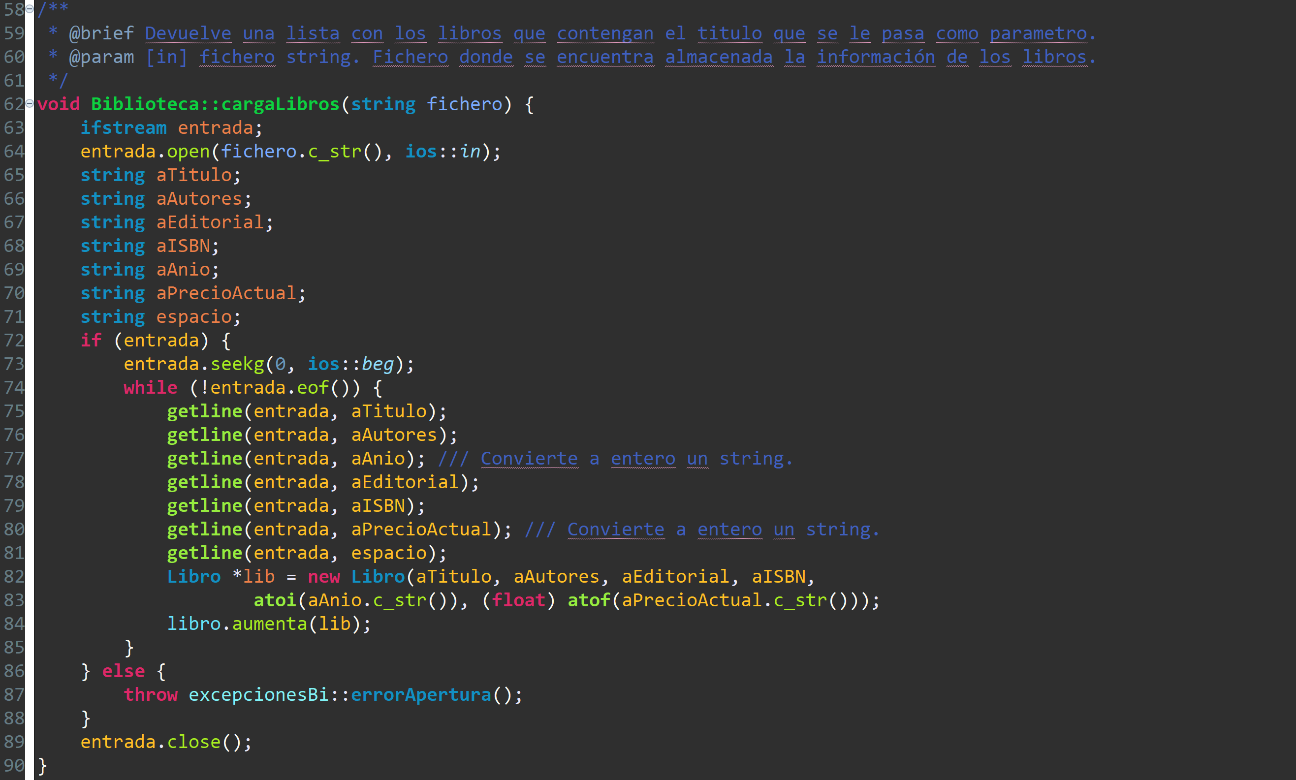
\includegraphics[scale=0.8]{img/img7.png}
				\caption{Captura de pantalla del cumplimiento del estándar FIO50-CPP.}
				\label{img7}
			\end{figure}
		
			\paragraph{}En esta solución compatible, la std::basic$\_$istream$<$T$>$::seekg() función se llama en la línea 73,  entre la salida y la entrada,  posicionando el puntero al comienzo de la lectura, eliminando el comportamiento indefinido .
		
	\subsection{FIO51-CPP. Cerrar los archivos cuando ya no sean necesarios.}
	
		\subsubsection{Enlace al sitio web del estándar seleccionado}
	
			\paragraph{}\url{https://wiki.sei.cmu.edu/confluence/display/cplusplus/FIO51-CPP.+Close+files+when+they+are+no+longer+needed}
	
		\subsubsection{Explicación sobre su utilidad}
	
			\paragraph{}Una llamada a la función $std::basic\_filebuf<T>::open()$ siempre debe ir acompañada de otra llamada a la función $std::basic_filebuf<T>::close()$ antes de la finalización del ciclo de vida del último puntero que almacenase el valor devuelto por la llamada de la primera función ó antes de la finalización del programa, lo que ocurriese antes.
	
			\paragraph{}La mala praxis de este estándar puede provocar la utilización innecesaria de memoria estática durante toda la ejecución del programa. En el peor de los casos si se abrieran muchos archivos y no se cerrara ninguno durante la ejecución del programa, podría llegar a provocar un desbordamiento de la memoria estática. Aún utilizando memoria dinámica, si no cerramos el archivo cuando ya no sea necesario, seguiríamos desperdiciando memoria igualmente.
	
		\subsubsection{Aplicación del estándar al proyecto}
	
			\paragraph{}En el proyecto elegido para la realización de las prácticas solo se hace lectura de un fichero en una única función en todo el programa, esta función es "$void Biblioteca::cargaLibros(string fichero)$".
	
			\begin{figure}[H]
				\centering
				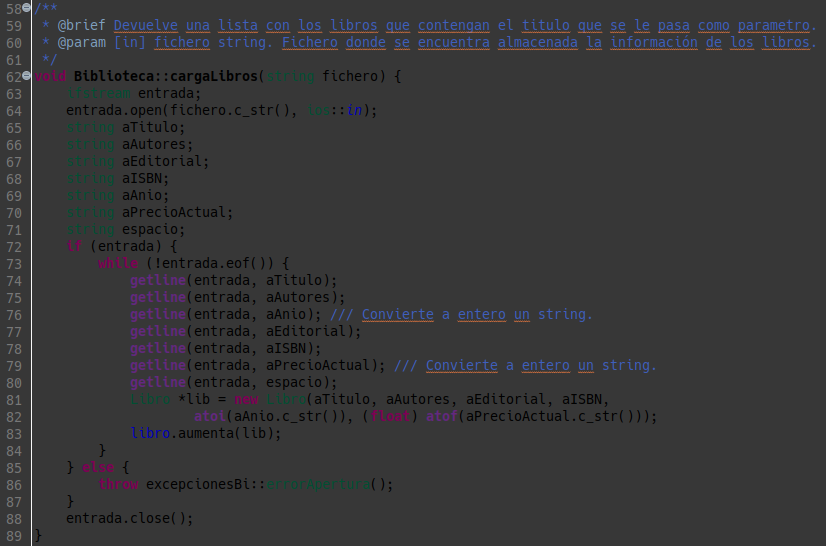
\includegraphics[scale=0.55]{img/captura1.png}
				\caption{Captura de pantalla del cumplimiento del estándar FIO51-CPP.}
				\label{captura1}
			\end{figure}
	
			\paragraph{}En la captura de pantalla anterior observamos que en la línea número 64 se abre el archivo "fichero" y, cuando ya se han realizado todas las operaciones de lectura del contenido del mismo, se procede a su cierre en la línea 88, quedando verificado el cumplimiento del estándar.
			
	\subsection{ERR51-CPP. Manejar todas las excepciones.}
	
		\subsubsection{Enlace al sitio web del estándar seleccionado}
			
			\paragraph{}\url{https://wiki.sei.cmu.edu/confluence/display/cplusplus/ERR51-CPP.+Handle+all+exceptions}
			
		\subsubsection{Explicación sobre su utilidad}
		
			\paragraph{}Cuando se produce una excepción, el control se transfiere al controlador más cercano con un tipo que coincide con el tipo de la excepción producida. Si no se encuentra ningún controlador coincidente directamente dentro de los controladores para un bloque try en el que se produce la excepción, la búsqueda de un controlador coincidente continúa buscando dinámicamente controladores en los bloques de prueba circundantes del mismo subproceso.
			
			\paragraph{}Todas las excepciones producidas por una aplicación deben ser detectadas por un controlador de excepciones coincidente. Incluso si la excepción no se puede recuperar correctamente, el uso del controlador de excepciones coincidente garantiza que la pila se desenrollará correctamente y proporciona la oportunidad de administrar correctamente los recursos externos antes de finalizar el proceso.
			
		\subsubsection{Aplicación del estándar al proyecto}
		
			\paragraph{}Aquí podemos ver como se lanzan excepciones, pero no son tratadas correctamente:
			
			\begin{figure}[H]
				\centering
				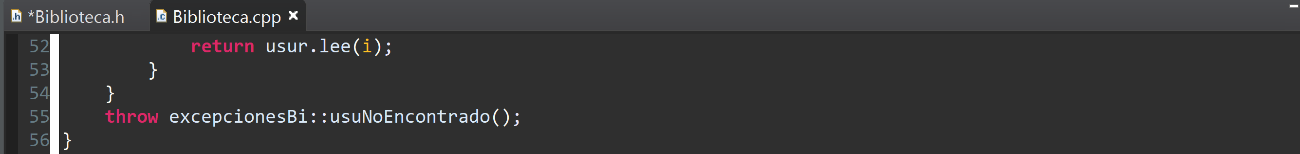
\includegraphics[scale=0.8]{img/img8.png}
				\caption{Captura de pantalla del incumplimiento del estándar ERR51-CPP.}
				\label{img8}
			\end{figure}
		
			\begin{figure}[H]
				\centering
				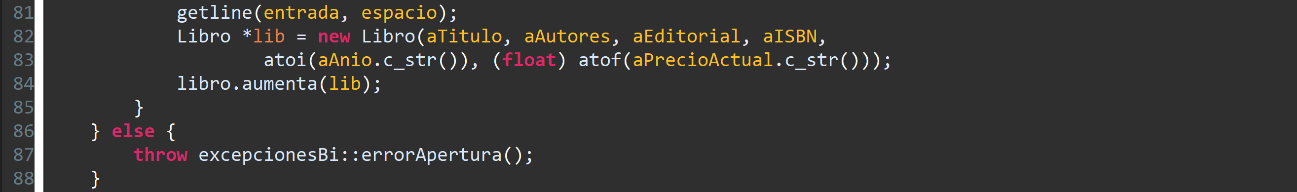
\includegraphics[scale=0.8]{img/img9.png}
				\caption{Captura de pantalla del incumplimiento del estándar ERR51-CPP.}
				\label{img9}
			\end{figure}
			
			\paragraph{}Ya que las clases no derivan de la clase exception ni tienen nada definido para ellas:
			
			\begin{figure}[H]
				\centering
				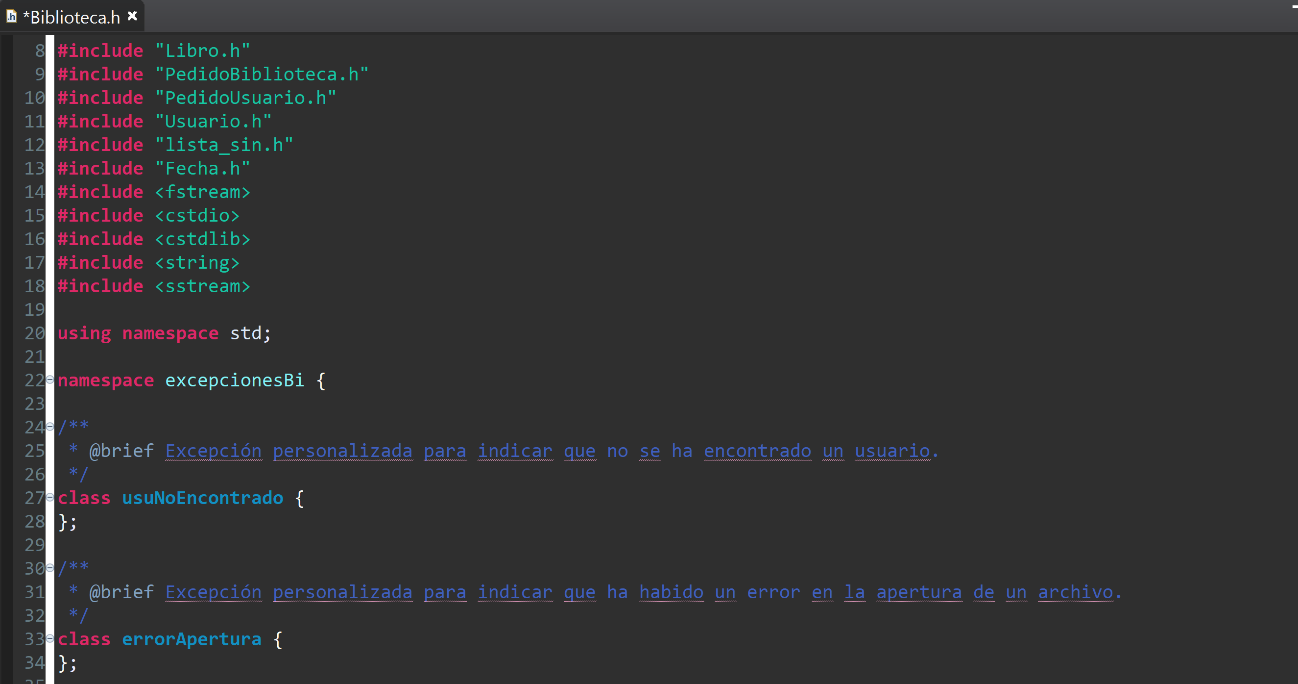
\includegraphics[scale=0.8]{img/img10.png}
				\caption{Captura de pantalla del incumplimiento del estándar ERR51-CPP.}
				\label{img10}
			\end{figure}
			
			\paragraph{}Una vez le hemos dado definición a dichas excepciones y con la inclusión de la directiva $\#$include $<$exception$>$ en el fichero de cabecera, ya podemos controlar las excepciones, lo que garantiza que la pila se desenrolla hasta la función y permite una gestión elegante de los recursos externos.
			
			\begin{figure}[H]
				\centering
				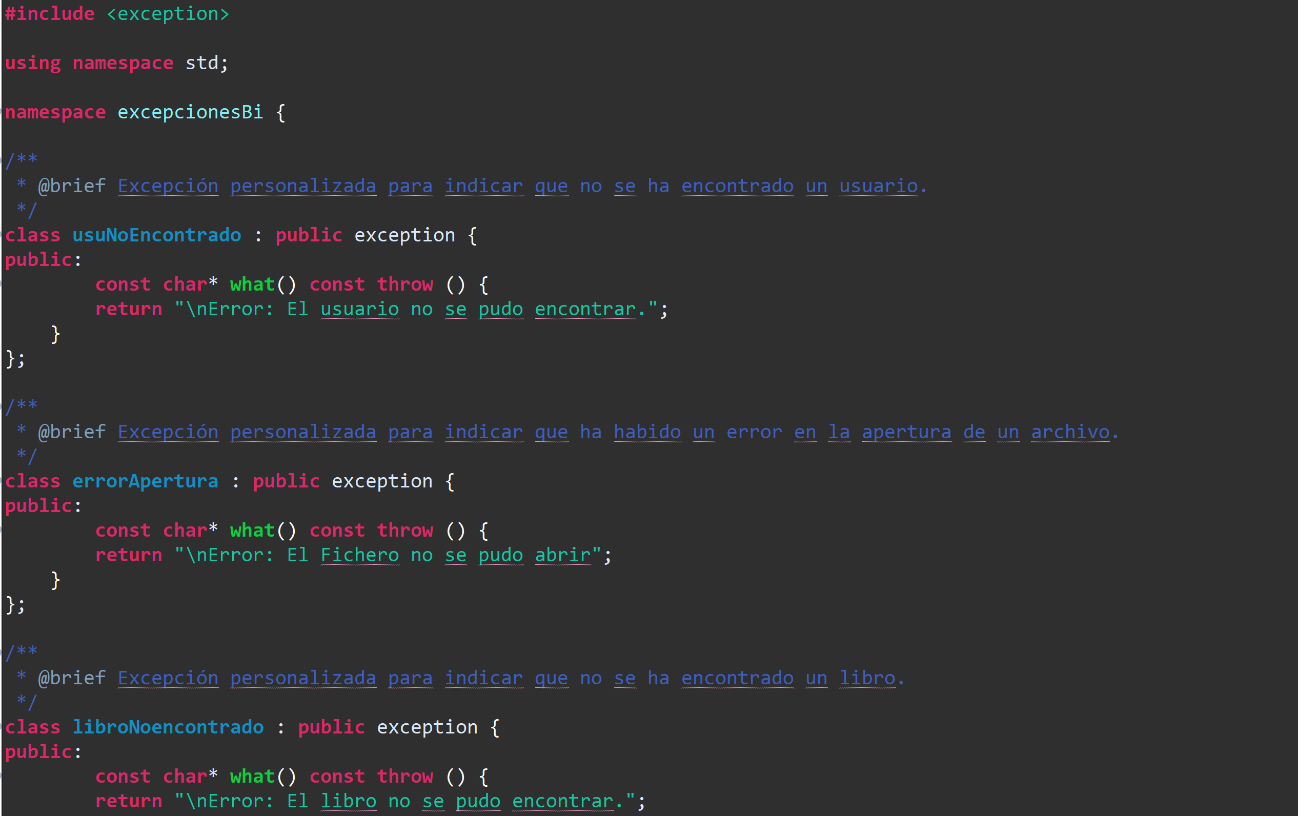
\includegraphics[scale=0.8]{img/img11.png}
				\caption{Captura de pantalla del cumplimiento del estándar ERR51-CPP.}
				\label{img11}
			\end{figure}
			
			\paragraph{}Se atrapan las excepciones lanzadas por los throw en los bloques catch pero no se tratan adecuadamente.
			
			\begin{figure}[H]
				\centering
				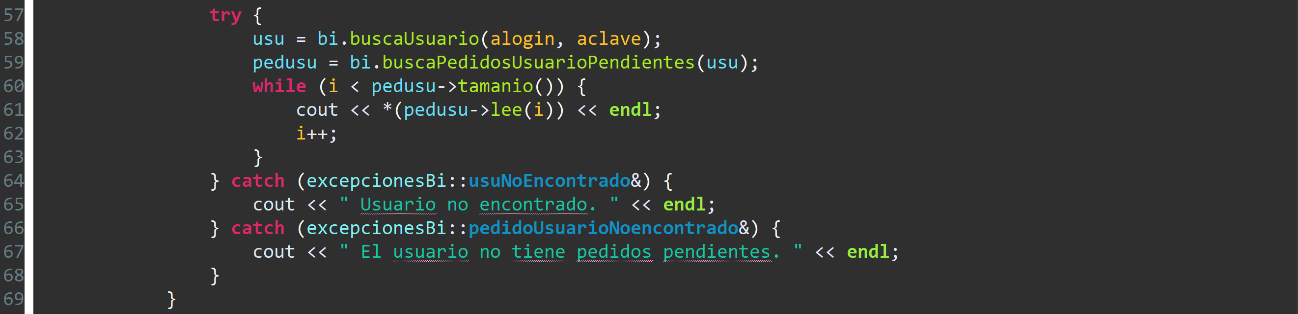
\includegraphics[scale=0.8]{img/img12.png}
				\caption{Captura de pantalla del incumplimiento del estándar ERR51-CPP.}
				\label{img12}
			\end{figure}
			
			\paragraph{}Y ya aquí se atrapan en el catch correspondiente y se tratan adecuadamente.
			
			\begin{figure}[H]
				\centering
				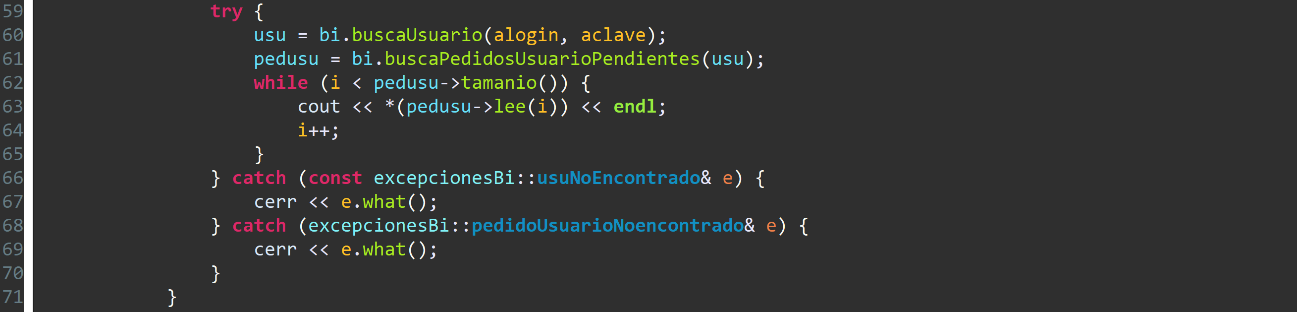
\includegraphics[scale=0.8]{img/img13.png}
				\caption{Captura de pantalla del cumplimiento del estándar ERR51-CPP.}
				\label{img13}
			\end{figure}
	
	\subsection{OOP53-CPP. Escribir los inicializadores de miembros de los constructores en el orden canónico.}
	
		\subsubsection{Enlace al sitio web del estándar seleccionado}
		
			\paragraph{}\url{https://wiki.sei.cmu.edu/confluence/display/cplusplus/OOP53-CPP.+Write+constructor+member+initializers+in+the+canonical+order}
		
		\subsubsection{Explicación sobre su utilidad}
		
			\paragraph{}Este estándar nos dice que la lista de inicializadores de miembros para un constructor permite que los miembros se inicialicen a valores especificados y que los constructores de clases base sean llamados con argumentos específicos.
			
			\paragraph{}Es decir, en el caso de que un atributo miembro de la clase necesite el valor de otro atributo miembro, este debe de estar inicializado previamente. El atributo miembro dependiente irá después del miembro del que depende en la lista de atributos y en el constructor.
			
			\paragraph{}En el caso de que no se cumpliera este estándar y en el constructor el miembro dependiente se intentara inicializar antes de que se haya inicializado el miembro del que depende, daría lugar a un comportamiento indefinido, como por ejemplo leer memoria no inicializada (datos basura).
			
			\paragraph{}En definitiva, se deben de escribir siempre los inicializadores de miembros en un constructor en el orden canónico: primero las clases base directas en el orden en que aparecen en la lista de especificador-base para la clase, luego los miembros de datos no estáticos en el orden en que se declaran en la definición de la clase.
		
		\subsubsection{Aplicación del estándar al proyecto}
		
			\paragraph{}En nuestro proyecto se encuentran las siguientes clases:
			
			\begin{itemize}
				\item Aplication
				\item Biblioteca
				\item Fecha
				\item Libro
				\item lista$\_$sin
				\item PedidoBiblioteca
				\item PedidoUsuario
				\item Usuario
			\end{itemize}
		
			\paragraph{}Para la clase Aplication, tenemos la siguiente lista de miembros:
			
			\begin{figure}[H]
				\centering
				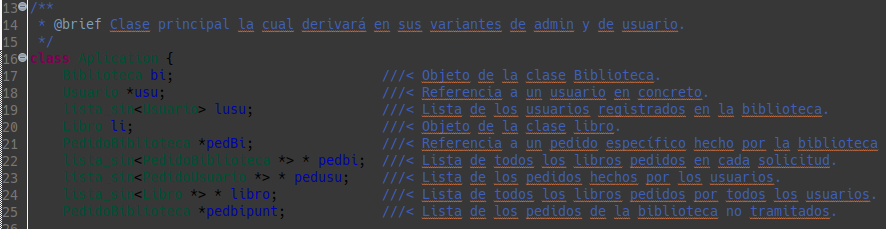
\includegraphics[scale=0.55]{img/captura2.png}
				\caption{Captura de pantalla de los atributos miembros de la clase Aplication.}
				\label{captura2}
			\end{figure}
		
			\paragraph{}En la siguiente captura de pantalla se puede apreciar cómo no se cumple claramente con el estándar, ya que la inicialización de los atributos miembros de la clase no siguen el orden establecido en la declaración  de la clase y hay atributos que no se inicializan.
			
			\begin{figure}[H]
				\centering
				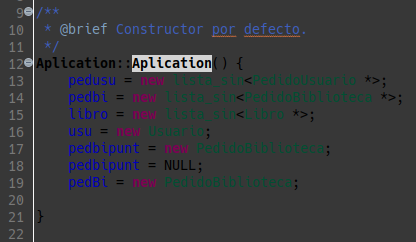
\includegraphics[scale=0.7]{img/captura3.png}
				\caption{Captura de pantalla del incumplimiento del estándar OOP53-CPP.}
				\label{captura3}
			\end{figure}
		
			\paragraph{} A continuación, se ha incluido la inicialización de los atributos que no aparecían y se han inicializado todos los atributos en el orden con el que se declaran en la clase:
			
			\begin{figure}[H]
				\centering
				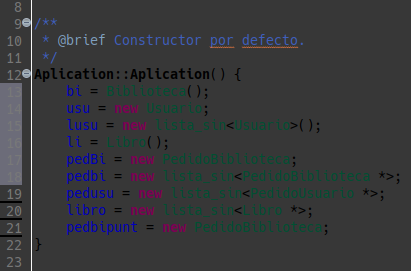
\includegraphics[scale=0.7]{img/captura4.png}
				\caption{Captura de pantalla del cumplimiento del estándar OOP53-CPP.}
				\label{captura4}
			\end{figure}
		
				\paragraph{}Para la clase Biblioteca, tenemos la siguiente lista de miembros:
			
			\begin{figure}[H]
				\centering
				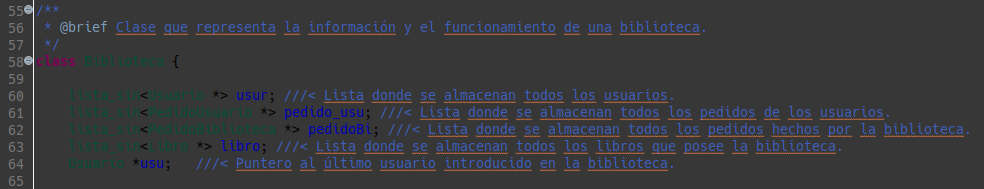
\includegraphics[scale=0.45]{img/captura5.png}
				\caption{Captura de pantalla de los atributos miembros de la clase Biblioteca.}
				\label{captura5}
			\end{figure}
		
			\paragraph{}En la siguiente captura de pantalla se puede apreciar cómo sí se cumple claramente con el estándar, ya que la inicialización de los atributos miembros de la clase siguen el orden establecido en la declaración  de la clase y se inicializan todos los atributos.
			
			\begin{figure}[H]
				\centering
				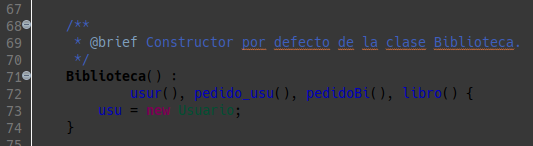
\includegraphics[scale=0.7]{img/captura6.png}
				\caption{Captura de pantalla del cumplimiento del estándar OOP53-CPP.}
				\label{captura6}
			\end{figure}
		
			\paragraph{}Para la clase Fecha, tenemos la siguiente lista de miembros:
			
			\begin{figure}[H]
				\centering
				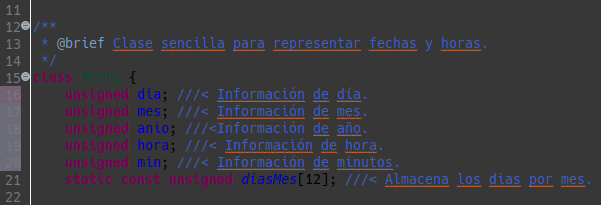
\includegraphics[scale=0.7]{img/captura7.png}
				\caption{Captura de pantalla de los atributos miembros de la clase Fecha.}
				\label{captura7}
			\end{figure}
		
			\paragraph{}En la siguiente captura de pantalla se muestra el código fuente del constructor por defecto de la clase. Se puede observar que se delega la inicialización de las variables en una función externa, por lo que daremos por no cumplido el estándar.
			
			\begin{figure}[H]
				\centering
				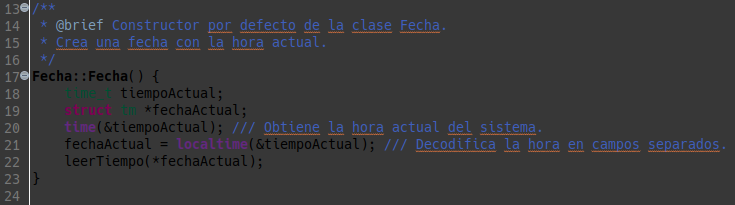
\includegraphics[scale=0.6]{img/captura8.png}
				\caption{Captura de pantalla en la que se muestra el incumplimiento del estándar OOP53-CPP.}
				\label{captura8}
			\end{figure}
		
			\paragraph{}Para corregirlo, añadimos la inicialización de los atributos miembros de la clase al final, en el orden de declaración de los mismos:
			
			\begin{figure}[H]
				\centering
				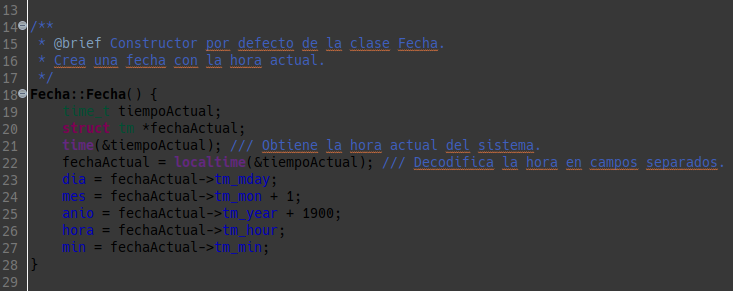
\includegraphics[scale=0.6]{img/captura9.png}
				\caption{Captura de pantalla en la que se muestra el cumplimiento del estándar OOP53-CPP.}
				\label{captura9}
			\end{figure}
		
			\paragraph{}Tanto para el constructor parametrizado como para el constructor por copia, se puede observar en las siguientes capturas de pantalla que se cumple con el estándar:
			
			\begin{figure}[H]
				\centering
				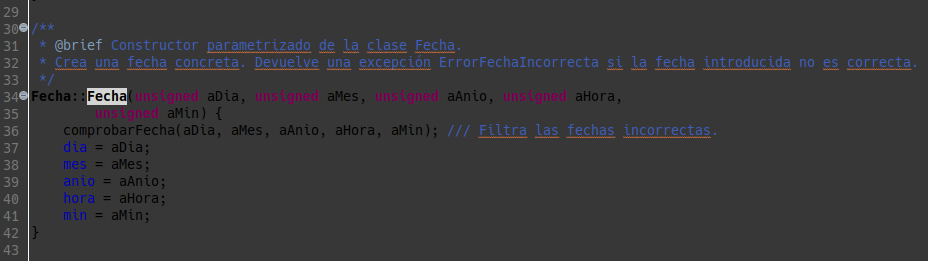
\includegraphics[scale=0.5]{img/captura10.png}
				\caption{Captura de pantalla en la que se muestra el cumplimiento del estándar OOP53-CPP.}
				\label{captura10}
			\end{figure}
		
			\begin{figure}[H]
				\centering
				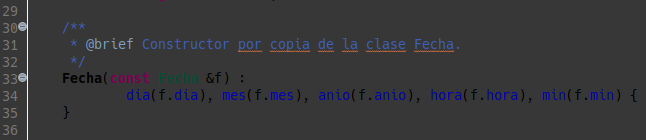
\includegraphics[scale=0.7]{img/captura11.png}
				\caption{Captura de pantalla en la que se muestra el cumplimiento del estándar OOP53-CPP.}
				\label{captura11}
			\end{figure}
		
			\paragraph{}Para la clase Libro, tenemos la siguiente lista de miembros:
			
			\begin{figure}[H]
				\centering
				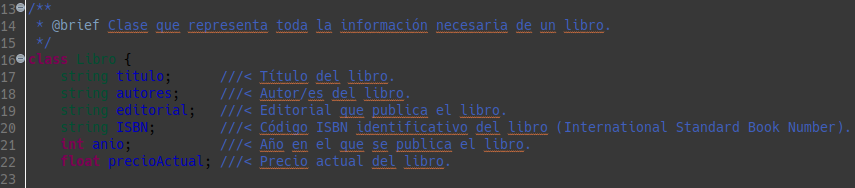
\includegraphics[scale=0.55]{img/captura12.png}
				\caption{Captura de pantalla de los atributos miembros de la clase Libro.}
				\label{captura12}
			\end{figure}
		
			\paragraph{}En la siguiente captura de pantalla se puede comprobar que en el constructor por defecto de la clase no se cumple el estándar, ya que no respeta el orden de los atributos miembros de la clase:
			
			\begin{figure}[H]
				\centering
				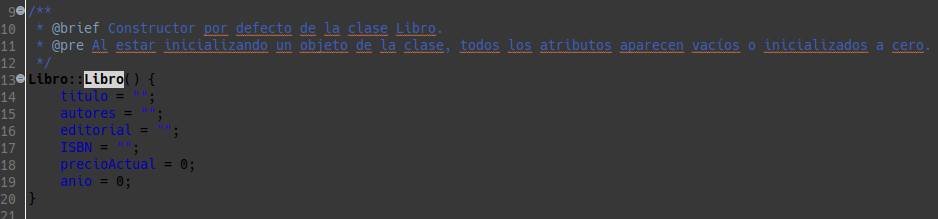
\includegraphics[scale=0.5]{img/captura13.png}
				\caption{Captura de pantalla en la que se muestra el incumplimiento del estándar OOP53-CPP.}
				\label{captura13}
			\end{figure}
		
			\paragraph{}Esto se soluciona reordenando la inicialización en el orden correcto:
			
			\begin{figure}[H]
				\centering
				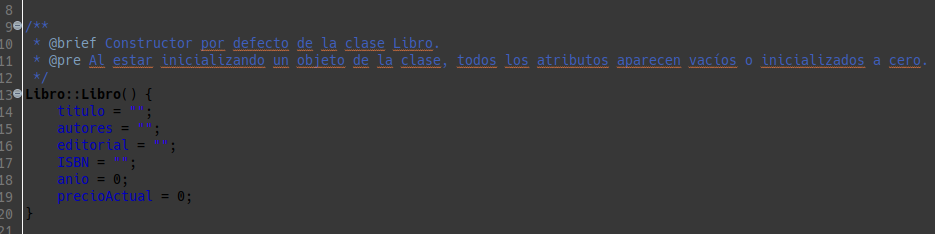
\includegraphics[scale=0.5]{img/captura14.png}
				\caption{Captura de pantalla en la que se muestra el cumplimiento del estándar OOP53-CPP.}
				\label{captura14}
			\end{figure}
		
			\paragraph{}Para el constructor parametrizado y el constructor por copia observamos que sí se cumple el estándar:
			
			\begin{figure}[H]
				\centering
				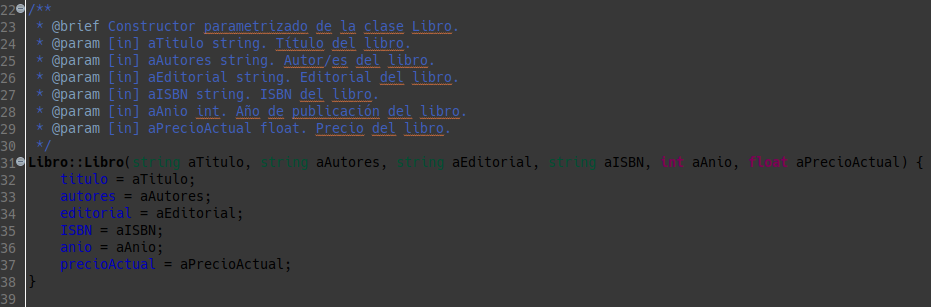
\includegraphics[scale=0.5]{img/captura15.png}
				\caption{Captura de pantalla en la que se muestra el cumplimiento del estándar OOP53-CPP.}
				\label{captura15}
			\end{figure}
		
			\begin{figure}[H]
				\centering
				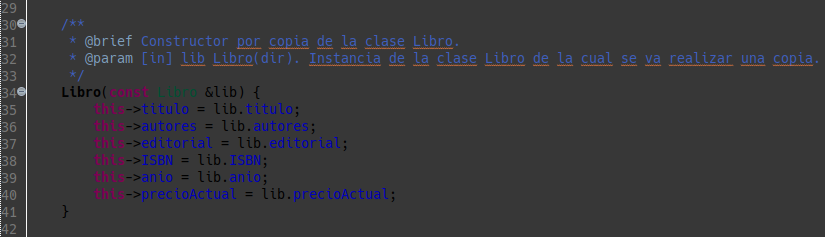
\includegraphics[scale=0.55]{img/captura16.png}
				\caption{Captura de pantalla en la que se muestra el cumplimiento del estándar OOP53-CPP.}
				\label{captura16}
			\end{figure}
		
			\paragraph{}Para la clase plantilla lista$\_$sin, tenemos la siguiente lista de miembros:
			
			\begin{figure}[H]
				\centering
				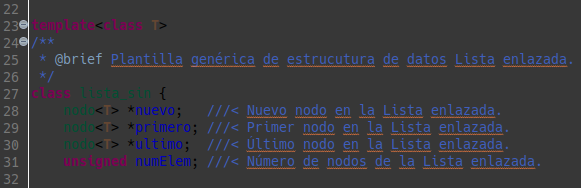
\includegraphics[scale=0.6]{img/captura17.png}
				\caption{Captura de pantalla de los atributos miembros de la clase lista$\_$sin.}
				\label{captura17}
			\end{figure}
			
			\paragraph{}Podemos observar en las siguientes capturas de pantalla que tanto el constructor por defecto como el constructor por copia cumplen con el estándar:
			
			\begin{figure}[H]
				\centering
				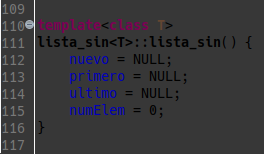
\includegraphics[scale=0.7]{img/captura18.png}
				\caption{Captura de pantalla en la que se muestra el cumplimiento del estándar OOP53-CPP.}
				\label{captura18}
			\end{figure}
			
			\begin{figure}[H]
				\centering
				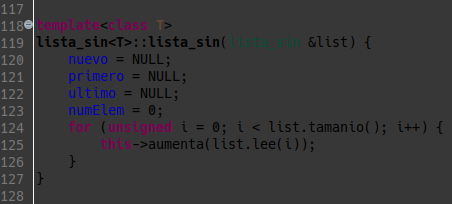
\includegraphics[scale=0.7]{img/captura19.png}
				\caption{Captura de pantalla en la que se muestra el cumplimiento del estándar OOP53-CPP.}
				\label{captura19}
			\end{figure}
		
			\paragraph{}Para la clase clase PedidoBiblioteca, tenemos la siguiente lista de miembros:
			
			\begin{figure}[H]
				\centering
				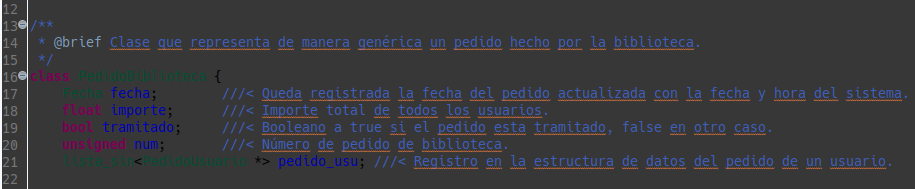
\includegraphics[scale=0.5]{img/captura20.png}
				\caption{Captura de pantalla de los atributos miembros de la clase PedidoBiblioteca.}
				\label{captura20}
			\end{figure}
		
			\paragraph{}El constructor por defecto, parametrizado y por copia de la clase no respetan el orden establecido de los atributos miembros, no cumpliendo de este modo con el estándar:
			
			\begin{figure}[H]
				\centering
				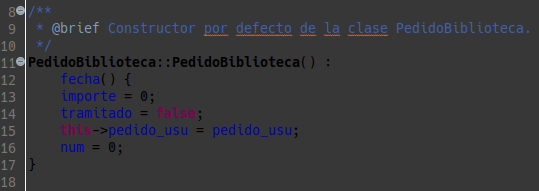
\includegraphics[scale=0.7]{img/captura21.png}
				\caption{Captura de pantalla en la que se muestra el incumplimiento del estándar OOP53-CPP.}
				\label{captura21}
			\end{figure}
		
			\begin{figure}[H]
				\centering
				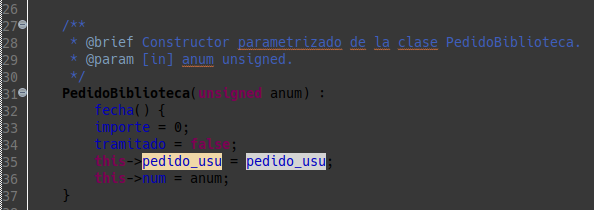
\includegraphics[scale=0.7]{img/captura22.png}
				\caption{Captura de pantalla en la que se muestra el incumplimiento del estándar OOP53-CPP.}
				\label{captura22}
			\end{figure}
		
			\begin{figure}[H]
				\centering
				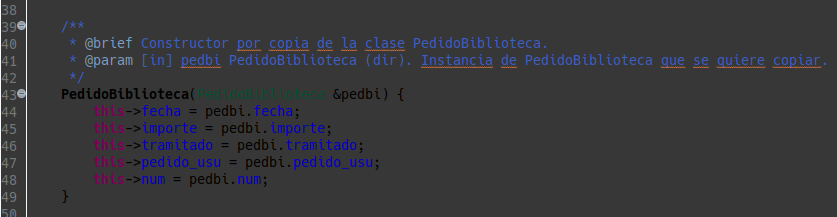
\includegraphics[scale=0.5]{img/captura25.png}
				\caption{Captura de pantalla en la que se muestra el incumplimiento del estándar OOP53-CPP.}
				\label{captura25}
			\end{figure}
		
			\paragraph{}Para poder cumplir con el estándar lo único que tenemos que hacer es ordenar la inicialización de los atributos del siguiente modo:
			
			\begin{figure}[H]
				\centering
				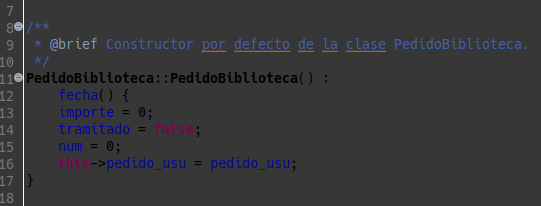
\includegraphics[scale=0.7]{img/captura23.png}
				\caption{Captura de pantalla en la que se muestra el cumplimiento del estándar OOP53-CPP.}
				\label{captura23}
			\end{figure}
			
			\begin{figure}[H]
				\centering
				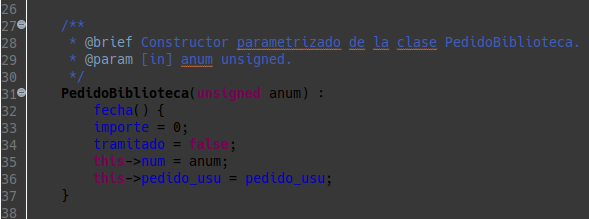
\includegraphics[scale=0.7]{img/captura24.png}
				\caption{Captura de pantalla en la que se muestra el cumplimiento del estándar OOP53-CPP.}
				\label{captura24}
			\end{figure}
		
			\begin{figure}[H]
				\centering
				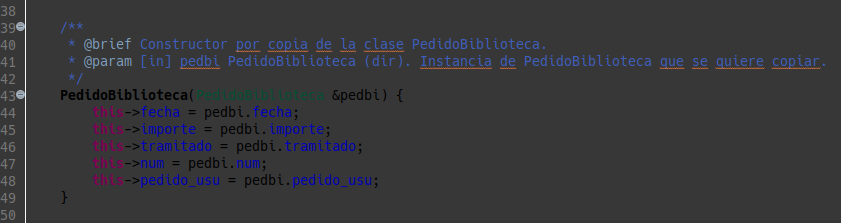
\includegraphics[scale=0.5]{img/captura26.png}
				\caption{Captura de pantalla en la que se muestra el cumplimiento del estándar OOP53-CPP.}
				\label{captura26}
			\end{figure}
		
			\paragraph{}Para la clase clase PedidoUsuario, tenemos la siguiente lista de miembros:
			
			\begin{figure}[H]
				\centering
				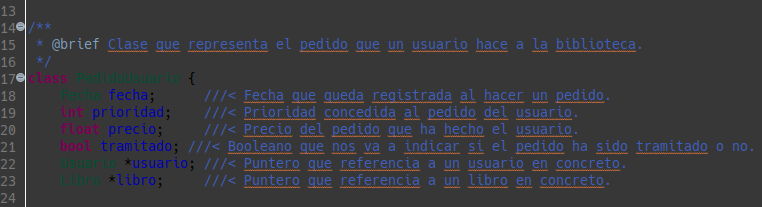
\includegraphics[scale=0.5]{img/captura27.png}
				\caption{Captura de pantalla de los atributos miembros de la clase PedidoUsuario.}
				\label{captura27}
			\end{figure}
		
			\paragraph{}Para los constructores por defecto y parametrizado podemos observar que no se cumple el estándar, como se puede observar en las siguientes capturas de pantalla:
			
			\begin{figure}[H]
				\centering
				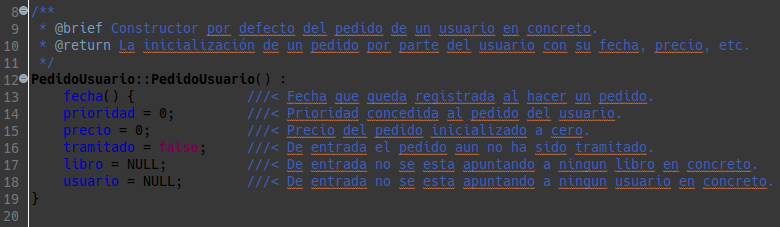
\includegraphics[scale=0.6]{img/captura28.png}
				\caption{Captura de pantalla en la que se muestra el incumplimiento del estándar OOP53-CPP.}
				\label{captura28}
			\end{figure}
		
			\begin{figure}[H]
				\centering
				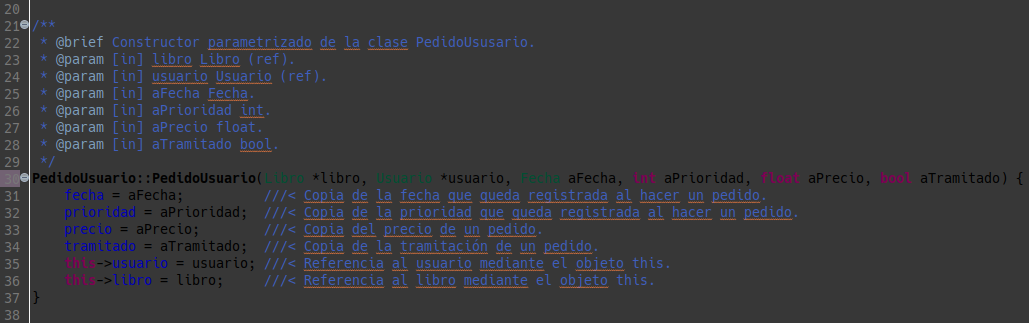
\includegraphics[scale=0.45]{img/captura30.png}
				\caption{Captura de pantalla en la que se muestra el incumplimiento del estándar OOP53-CPP.}
				\label{captura30}
			\end{figure}
		
			\paragraph{}Para hacer que se cumpla con el estándar, debemos inicializar los atributos miembros según el orden establecido en la declaración de la clase, como se muestra en las siguientes capturas de pantalla:
			
			\begin{figure}[H]
				\centering
				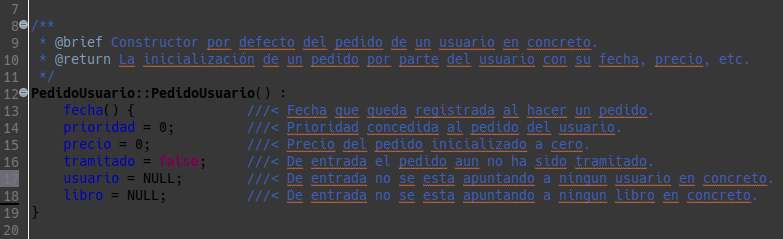
\includegraphics[scale=0.6]{img/captura29.png}
				\caption{Captura de pantalla en la que se muestra el cumplimiento del estándar OOP53-CPP.}
				\label{captura29}
			\end{figure}
		
			\begin{figure}[H]
				\centering
				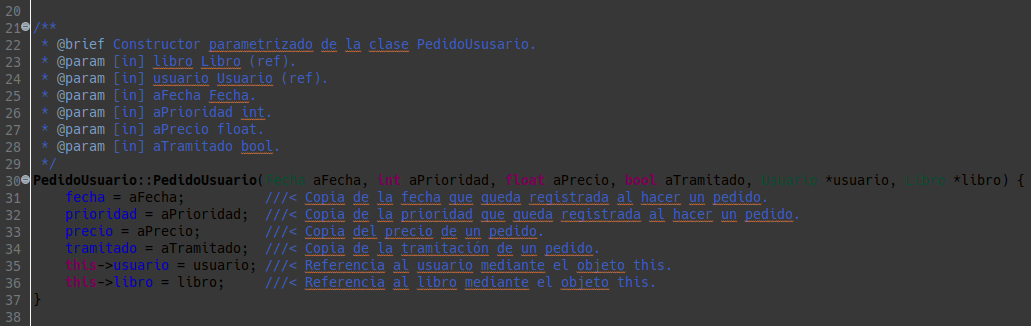
\includegraphics[scale=0.45]{img/captura31.png}
				\caption{Captura de pantalla en la que se muestra el cumplimiento del estándar OOP53-CPP.}
				\label{captura31}
			\end{figure}
		
			\paragraph{}Para la clase clase Usuario, tenemos la siguiente lista de miembros:
			
			\begin{figure}[H]
				\centering
				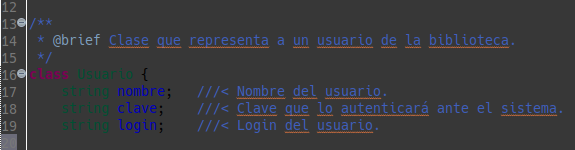
\includegraphics[scale=0.8]{img/captura32.png}
				\caption{Captura de pantalla de los atributos miembros de la clase Usuario.}
				\label{captura32}
			\end{figure}
		
			\paragraph{}En el caso de esta clase, solo se dispone de un constructor por defecto. En este, no se respeta el estándar ya que no se inicializan los atributos miembro en el orden canónico, como se puede observar en la siguiente captura de pantalla:
			
			\begin{figure}[H]
				\centering
				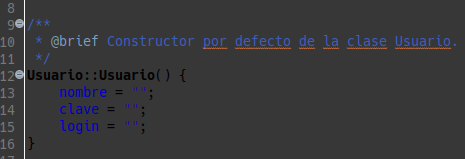
\includegraphics[scale=0.9]{img/captura33.png}
				\caption{Captura de pantalla en la que se muestra el incumplimiento del estándar OOP53-CPP.}
				\label{captura33}
			\end{figure}
			
			
		
	\subsection{MSC52-CPP. Las funciones que devuelven un valor deben devolver un valor desde todas las rutas de salida.}
	
		\subsubsection{Enlace al sitio web del estándar seleccionado}
		
			\paragraph{}\url{https://wiki.sei.cmu.edu/confluence/display/cplusplus/MSC52-CPP.+Value-returning+functions+must+return+a+value+from+all+exit+paths}
		
		\subsubsection{Explicación sobre su utilidad}
		
			\paragraph{}La utilidad de la aplicación de este estándar es bastante conocida. Este estándar nos dice que, siempre que una función devuelve un valor, cada ruta de ejecución de la misma debe de devolver siempre un valor. En el caso de que en algún caso no se devolviera nada, esto podría desembocar en un comportamiento indefinido de la aplicación.
		
		\subsubsection{Aplicación del estándar al proyecto}
		
			\paragraph{}En nuestro proyecto, todas las funciones que devuelven un valor cumplen con este estándar. Dentro de las funciones que devuelven un valor, en nuestro proyecto hay tres tipos diferenciados: las funciones que solo tienen una ruta de ejecución, las funciones que tienen más de una ruta de ejecución y devuelven un valor en cada ruta, y las funciones que tienen más de una ruta de ejecución pero no devuelven un valor en todas.
			
			\paragraph{}Las funciones que solo tienen una ruta de ejecución las obviaremos en este informe, ya que el cumplimiento de este estándar resulta algo trivial de comprobar.
			
			\paragraph{}Para el segundo tipo de funciones pondremos un par de ejemplos a continuación en los que se puede comprobar claramente que no existe ninguna ruta de ejecución en la que no se devuelva ningún valor.
			
			\begin{figure}[H]
				\centering
				\includegraphics[scale=0.45]{img/captura34.png}
				\caption{Captura de pantalla del cumplimiento del estándar MSC52-CPP.}
				\label{captura34}
			\end{figure}
		
			\begin{figure}[H]
				\centering
				\includegraphics[scale=0.45]{img/captura35.png}
				\caption{Captura de pantalla del cumplimiento del estándar MSC52-CPP.}
				\label{captura35}
			\end{figure}
		
			\paragraph{}Para el tercer tipo de funciones, si bien no se devuelve un valor en alguna de las rutas de ejecución, esto es debido a que la devolución de un valor no válido produciría un error de ejecución. Por este motivo, no se devuelve un valor sino que se ejecuta una excepción que detiene la ejecución para evitar comportamientos impredecibles.
			
			\paragraph{}Teniendo en cuenta lo anterior, en el resto de rutas de ejecución que no causan excepciones sí se devuelve siempre un valor. Por este motivo, se considera cumplido el estándar. A continuación, dejamos un par de capturas de funciones de este tipo: 
			
			\begin{figure}[H]
				\centering
				\includegraphics[scale=0.5]{img/captura36.png}
				\caption{Captura de pantalla del cumplimiento del estándar MSC52-CPP.}
				\label{captura36}
			\end{figure}
			
			\begin{figure}[H]
				\centering
				\includegraphics[scale=0.45]{img/captura37.png}
				\caption{Captura de pantalla del cumplimiento del estándar MSC52-CPP.}
				\label{captura37}
			\end{figure}

	

\newpage